\openingarticle
\def\ppages{\pagerange{davis:firstpage}{davis:lastpage}}
\def\authormail{ddavis17@binghamton.edu}
\def\shorttitle{An Analysis of the Roman Agroeconomy}
\def\maintitle{Tetra-dimensional Climate and its Effects  
	on the Roman State: An Archaeological Analysis of the 
	Roman Agroeconomy}
\def\shortauthor{Dylan Davis}
\def\thanknote{\footnote{Dylan Davis attends Binghamton University, in New York State, USA. He is double majoring with a BS in Anthropology and a BA in Geography, specialising in archaeology and computer applications in human environmental analysis. His archaeological interests include human-environmental interactions and their relation to social development and collapse. He will be attending graduate school after completing his undergraduate studies, and will be focusing his MA thesis on Easter Island, incorporating geo-spatial analysis and environmental archaeology.}}
\def\affiliation{Binghamton University (USA)}
%--------------------------------------------------------------
\mychapter{Tetra-dimensional Climate and its Effects  
	on \\the Roman State: An Archaeological Analysis of the 
	Roman Agroeconomy}
\begin{center}
	{\Large\scshape\shortauthor \thanknote}\\[1em]
	\email \\%[.5em]
	\affiliation
\end{center}
\vspace{3em}
\midarticle
%--------------------------------------------------------------
\label{davis:firstpage}

	%----------------------------------------------------------------------------------------
	%	ABSTRACT
	%----------------------------------------------------------------------------------------
	\begin{myabstract}
This\marginnote{Abstract\\ (In French and Italian see below)} paper examines the relationship between environmental vacillation and the success of societal institutions in the Roman Empire, specifically the economy. A detailed investigation exploring the rise of the Roman economy is undertaken through the use of archaeological and climatological evidence. Climate, as defined in this paper, consists of four parts –environmental climate, social climate, economic climate, and political climate– thus establishing the Tetra-dimensional Climate Model. The results of this study indicate a strong relationship between the rise of agriculture and the rise of maritime trade during the Roman Republic and the Roman Empire. This increase in agricultural production was largely a result of climatological stability in Europe, as well as the temporary tranquillity of the political climate following the foundation of Rome. As political and social stability vacillated throughout Rome’s years in power, economic development -- especially in the agricultural sector -– also changed course.


		\keywords[Keywords]{Classical Archaeology, Roman Economy, Maritime Trade, Environmental Archaeology, Nautical Archaeology.}
	\end{myabstract}
	

		
	%----------------------------------------------------------------------------------------
	%	ARTICLE CONTENTS
	%----------------------------------------------------------------------------------------
	
%	\section{Introduction}

	\lettrine[nindent=0em,lines=3]{B}{eginning} as early as the \nth{6} century BC, 
farms began to emerge throughout the Italian countryside\footnote{The Oxford Roman Economy Project, of which much of the following data is based, “addresses the fundamentals of the Roman imperial economy and analyses all major economic activities (including agriculture, trade, commerce, and extraction), utilising quantifiable bodies of archaeological and documentary evidence and placing them in the broader structural context of regional variation, distribution, size and nature of markets, supply and demand.”}. 
As time passed, these farms grew in size, and eventually transformed into agricultural institutions: vineyards, villas, and high-yielding production zones.\footnote{When referring to farms, villas, and estates, the following should be considered: farms are the smallest, usually referring to land run by a single family; villas (in this instance, agricultural villas) are usually owned by a wealthy individual or family and are run by servants or slaves; estates are in many ways similar to villas but generally include more farmable land.} 
Many of these large estates were owned -- or at least partially owned -- by the wealthy, landowning elite of the Roman world. Some of these aristocratic Romans were senators, such as Scipio Africanus, who owned a vineyard next to his villa in Liternum, and L. Sestius, who owned villas that flourished on exporting wines throughout the Adriatic \parencite[6, 16]{Purcell_1985}. However, not all wealthy landowners were members of the Senate. The rise in number of such estates coincided with an increase in trade, which can be further witnessed in the distribution of amphorae, an increase in the production of coinage, and a spike in maritime traffic, leading to higher rates of shipwrecking \parencites{Manacorda_1978}{Hopkins_1980}. A high rate of association between the emergence of large-scale agricultural production and a peak in Mediterranean trade is seen through statistical analysis of agricultural presses, shipwrecking, and coinage production. 
	
	Yet, what caused this spike in agricultural production? Surely it was more than just the appearance of large estates and the rise of the Roman landowning elite. What were the factors that allowed for this rapid expansion of the Roman agricultural sector? The various elements that permitted for an unprecedented rise in the number of farms and agricultural estates can be compiled into one category: climatological stability. 

	This article seeks to put forth a new definition of climate by breaking the term into four different subgroups: societal climate, economic climate, political climate, and environmental climate. Tetra-dimensional climate creates a general variable that is responsible for the success or failure of nearly every human institution in a given society. Most pivotal moments in the history of humankind can be traced back to the climatological context of the time, whether it is the societal climate, the political climate, the economic climate, or the environmental climate. Each individual variable can have effects on human society, and the more of these variables that are in oscillation, the more likely anthropological change is to occur. 
	
	Societal organisations can be easily understood when looking at systems in other aspects of the natural world. In an ecological context, every member of a society has a crucial role, and any small change can, and will, have impacts on the system as a whole. In order for the system to sustain itself, it has to be resilient, adaptive, and transformative to changing conditions \parencite{Walker_2004}. Forces that impact the ecology of human organisations consist of the four components of climate discussed previously, and resilience, adaptability, and transformation are essential to survival. When the climatological tetrad is favourable – agricultural production is high, economies are thriving, social tensions are low, and political systems effectively keep their citizens protected and content – then human society thrives and expands.\footnote{For a good reference for the factors that encourage and inhibit the expansion of human civilisation, see \textcite{Diamond_1997}.} 
However, when the tetrad is unfavourable – poor harvests; economic collapse; lack of available resources; corrupt, tyrannical, or ineffective political systems – then human society tends to fall into chaos. \footnote{Favourable and unfavourable environmental climates can be detected archaeologically through environmental proxies, historical records, and archaeological remains. When there is evidence for massive violence, destruction, or famine, the climatological tetrad may have been in flux. At the same time, if there is evidence of prolonged residency in a region, an abundance of resources, and a myriad of building projects, then the environments were likely favourable.} Granted, in some instances, societies cope in positive ways to these climatic challenges, and this anarchic outcome is avoided altogether. Nonetheless, in extreme and prolonged circumstances, civilisations tend to dissolve in the presence of such problems. 
The Roman Empire is no exception to this pattern, and through the use of the Tetra-dimensional Climate Model, it is demonstrated that during periods of environmental climate change that led to agricultural failures, the economic and political sectors also began to fail. These collapses left society in a state of uncertainty. 

%\section{The Tetra-Dimensional Climate Model}
As\marginnote{The Tetra-Dimensional Climate Model} mentioned previously, the tetra-dimensional climate model (TDCM) consists of four components. These pieces together form one variable that is indicative of the success or failure of a given human society. Let us now break down the TDCM into its various elements.

%\subsection{Environmental Climate}
The\marginnote{Environmental Climate} environmental climate is the traditional definition of climate, the influence or the environmental conditions characterising an area or a period. This is perhaps the component of TDCM that is most independent from human control in pre-industrial societies. Humans may alter the environment intentionally or unintentionally, but they cannot change weather patterns to “control” nature. As a result, the environmental climate of a region or time period generally dictates the direction that human civilisation will take, with environments favouring agricultural production being the most beneficial for human growth. 

%\subsection{Economic Climate}
The\marginnote{Economic Climate} economic climate of a group or region does not necessarily fall in line with modern economic theory. Ancient societies did not have a global economic system as we do today, and so “economics” in these instances simply refers to any occurrences of exchange between different groups. In the case of Rome, as well as many archaic societies, agricultural trade is among the first such elements of an “economy.” As a society becomes more advanced, economics may include the extraction of raw materials – such as precious metals and architectural materials including stone and marble – and widespread trading networks. When exchange between regions is constant/growing and tranquil, then the economic climate can be considered positive. If trade relations are virtually non-existent or in rapid decline, then the economic climate can be considered negative and thus a stymie to societal development.

%\subsection{Political Climate}
When\marginnote{Political Climate} defining political climate, stability and governmental system type are important determinants. For example, a totalitarian dictatorship issues an oppressive political climate, which is unsuitable for societal advancement. Democratic governments, on the other hand, allow for more social development. However, if the system of government, regardless of its type, is unstable (e.\,g. constant coup attempts, death of a leader, succession uncertainty), then the political climate is also unfavourable for human development. Therefore, the political climate is only beneficial when the system is stable and the governmental type is tolerant of societal innovation. 

%\subsection{Social Climate}
The\marginnote{Social Climate} overall consensus among the masses regarding their views of the political and economic systems in place is the best way to define social climate. For example, if a group of people find their government oppressive and their rights restricted, the social climate is one of contempt and will likely lead to a revolution or rebellion against the current political regime. Likewise, if the masses are unhappy with the economic climate (due to inflation, job availability, etc.), then the social climate will also be one of unrest. If the political and economic climates are both preventing social mobility or development, then the social climate will not only be negative, but will likely turn violent.

%\section{Methodology}
Unlike\marginnote{Methodology} many other theories relating to “climate”, TDCM combines multiple aspects of climate and aims to explain how human society is limited by environmental forces in addition to our own societal systems. Through the analysis of environmental proxies (e.g. dendrochronology and ice cores), a concise record of past environmental fluctuations was determined. For this study, tree-ring investigations by \textcite{Büntgen_2011a} and in \textcite{Büntgen_2011b}\footnote{The dendrochronological study used 
\num{7284} European oak tree samples and Alpine conifer data, in conjunction with \num{1089} stone pine and \num{457} European larch samples from the Austrian Alps. 
The samples allowed \textcite{Büntgen_2011a} to reconstruct the precipitation record for April through June and the temperature record June through August for the past 2500 years of European environmental history.}, and ice core analyses by \textcite{McCormick_2012} serve as the foundational data for reconstructing the environmental climate present during Rome’s expansion. In order to establish the state of the economic climate, statistical and geographical data relating to shipwrecking, coinage manufacturing, and agricultural production were used, in conjunction with archaeological evidence in the form of underwater and terrestrial discoveries (shipwrecks and their cargo and agricultural production centres, respectively). This evidence, when synthesised, helps to paint a picture of economic evolution throughout the history of the Roman Republic and Roman Empire. The political and social climates are investigated primarily through historical sources and are very often reflected in the economic climate of the corresponding time period. What is noticeable is that the three anthropological aspects of the climatic tetrad (economic, social, and political climate) are intertwined, whereas the environmental climate is not necessarily reciprocally influenced in the same way.

This paper is organised in chronological order, spanning from the \nth{6} and \nth{7} centuries\BC until the fall of Rome in the \nth{5} and \nth{6} centuries\AD. Within this chronological order, the elements of TDCM are highlighted and exemplified through archaeometric, archaeological, and geographical evidence.

%\section{The Rise of Farms and Villas}

After \marginnote{The Rise of Farms and Villas} the \nth{6} century\BC, pre-existing farms increased in size, changed ownership, and eventually transformed into massive villas and estates. Some of these land ownings were households for the elite with little to no agricultural significance. These villas can be seen as far back as the \nth{5} century\BC; yet, agricultural villas do not appear until the \nth{3} century\BC \parencite[18]{Terrenato_2001}. 
Originally, such large estates primarily functioned as aristocratic housing rather than lands for surplus agricultural production. Large, well-developed villas do not truly appear in abundance until the \nth{1} century\BC \parencite[24]{Terrenato_2001}. 
Historian Appian of Alexandria stated: “[t]he rich came to cultivate vast tracts instead of single estates” \parencite[98]{Potter_1990}. 
Although this record comes from the \nth{2} century\AD, it also accurately describes the \nth{2} century\BC in that during this time, villas and estates began to rise in their abundance.

Evidence for a surplus of agricultural production can be seen in the abundance of amphorae that begin to appear in the \nth{3} century\BC. 
By this time (and possibly a century or so earlier), Italian wine makers began to look beyond the local market to vend their products. 
In Naples, amphorae production increased from the second half of the \nth{4} century\BC “due to the diffusion of Aminea grapes within the area of the bay” \parencite[61]{Olcese_2005}. The fermented grape was a highly sought after commodity in antiquity because it was one of the most common sources of alcohol during this time period \parencite[2]{Purcell_1985}. In addition, wine was considered to be an “exotic item” by indigenous Europeans such as the Celts and did not spoil as quickly as locally produced beverages \parencite[383]{Dietler_1990}. 

As far back as the \nth{3} millennium\BC, there is evidence that wine was classified as an elite beverage, while beer remained the drink of commoners \parencite[233]{Dietler_2006}. 
Only within Greek and Italic societies did wine become the drink of the masses. 
The goods of viticulturists were soon shipped by sea within transport containers (amphorae) to sites throughout the Mediterranean \parencite[9]{Moore_1995}. 
These amphorae were based on Greek styles and were abundantly produced in the Italian provinces of Etruria, Latium, and Campania \parencite[285]{Woolf_1992}. 
Most of these amphorae contained wine\footnote{Campania is particularly famous for its wine production \parencite[6]{Purcell_1985}.}, and the Greco-Roman style amphora soon spread throughout the Mediterranean, including parts of Gaul, which formed a primary market for Italian wines \parencites[141]{Tchernia_2006}[7]{Purcell_1985}[285]{Woolf_1992}. In addition to the Greco-Roman style amphora, another type, known as Dressel~1, also originated in Italy and later replaced the Greco-Roman style in the mid-\nth{2} century\BC \parencites[263]{Peacock_1977}[285]{Woolf_1992}.\footnote{Dressel 1 containers are considered to be the first “truly Roman” form of amphorae \parencite[86]{Toscana_1995}.}. 
The increase in variety and number of amphorae throughout the Mediterranean evidences an increase in the production of wine and olive oil.\footnote{Olives were a staple of the Mediterranean diet because they are a good source of edible fat. 
In addition, olive oil could be used in soap or to fuel lamps \parencite[31]{Finley_1999}.} Nevertheless, most viticulture was not the result of production at large villas and estates, but rather small-scale farms and vineyards run by individuals, some of whom were not members of the Roman elite \parencites[163]{Kron_2012}[7]{Purcell_1985}. Peasants aimed to produce surpluses because without this buffer, in a bad year, they would starve \parencite[22]{Bowman_2013}. A surplus could be stored or sold – either to a middleman or in markets known as nundinae \parencite[113]{Storey_2004}.\footnote{Nundinae provided a convenient exchange mechanism for subsistence farmers in the countryside to sell their goods \parencite[113]{Storey_2004}.}.  These small-scale production centres were then connected with the Italic merchant class, who coordinated the exportation of the products that were harvested \parencites[47]{Kehoe_2013}[8]{Purcell_1985}. 

Regardless of the fact that small-scale production was at the forefront of these newly established trans-regional and trans-Mediterranean trade networks, the wealthy Italian elite soon began to consolidate their wealth in landholdings. The reasoning for this phenomenon is multifaceted. The consolidation of land appears related to a need for protection from Carthaginian forces during the Punic Wars, and the growth of a wealthy upper class seems to have led to the formation of latifundia – large estates that were run by slave labour –in Italy \parencite[98--106]{Potter_1990}. 
During the following centuries, villas began to appear in greater and greater numbers, especially in wine-producing regions. Around the late \nth{3} and \nth{2} centuries\BC, 
“the latifundia of the upper class became predominant in certain parts of the Italian countryside” \parencite[12]{Moore_1995}. This increasing prominence of the latifundia was the result of an influx of slave labour from prisoners of war \parencite[178--179]{Kay_2014}.  Large groupings of estates now began to cluster around notable areas such as Campania, Latium, and Etruria, which were known for their wine production. As a result, an agro-economy began to emerge throughout the Italian peninsula. Cicero writes, “but of all the occupations from which it is possible to make money, none is better than agriculture, none more productive, none sweeter, none more worthy of a free man” (cited in \textcite[133]{Kay_2014}). However, economic investment was only one of the reasons for a sudden rise in the number of villas and estates throughout Italy.\footnote{Chapter 7, “Investment Farming and Agricultural Exploitation”, in \textcite{Kay_2014} is a good resource for understanding agricultural systems in Roman Italy.} According to Nicola \textcite[29]{Terrenato_2001}, villas became exceedingly popular due to their profits made from supplying the army during times of war, dealing real-estate, the slave trade, and selling agricultural products such as oil, wine, olives, and grapes. In addition, villas were relatively stable investments that brought with them political and social influence, thus increasing the status and “respectability” of the owner \parencite[29]{Terrenato_2001}. \textcite[119]{Storey_2004} also states that the Roman elite became “heavily involved in commerce.” Therefore, social and political factors accompanied economic explanations in the rise of elite estates throughout the Italian peninsula and ubiquitously throughout the Roman Republic.

%\subsection{Applying Tetra-Climatological Theory}

When\marginnote{Applying Tetra-Climatological Theory} farms and villas began to proliferate within the whole of Italy in the \nth{6} century\BC, the Etruscans were still in a phase of expansion, and a plethora of city-states existed throughout the peninsula. Coalescentium – the gradual unification of small villages into larger city-states – dominated the political scene of the time. Farms that were formed were usually fairly small in size because of the constant threat of raids from neighbouring cities. When the Roman Republic was finally founded in 509\BC, stability in the immediate region soon followed, and a larger number of farms were established. Through the use of dendrochronology, \textcite{Büntgen_2011a} reconstructed temperature and precipitation records back to approximately 500\BC. Between 350\BC and 100\BC, temperature remains fairly stable throughout Europe, and precipitation levels rise steadily in each following century (Fig. \ref{fig:DavisFig1}). It is reasonable to assert that the rise in viticulture and olive oil production in many regions throughout Italy was, in part, due to the stable climatological conditions.
	
%FIGURE 1 HERE


Further evidence retrieved from the tree-ring study is seen in the levels of deforestation throughout Europe over the past 2500 years. There is an unequivocal rise in the amount of felling throughout the continent, beginning around 400\BC and peaking in the \nth{1} century\BC. As is evident from the dendrochronological studies conducted by \textcite[580]{Büntgen_2011a}, “onset of wetter and warmer summers is contemporaneous with the societal consolidation of new kingdoms.” The above average precipitation levels that were present from the Late Iron Age until  250\AD allowed for Celtic expansion and Roman conquest.\footnote{The average precipitation level, as calculated in \textcite{Büntgen_2011b}, 
was approximately \SI{210}{\milli\metre}. During Rome’s expansion around 250\BC, 
precipitation levels were approximately \SI{240}{\milli\metre}.} The pluvial conditions were complemented by increased, yet stable, temperatures. Later on, similar conditions allowed for kingdoms such as Francia -- which reached its peak under Charlemagne in the \nth{8} century – to expand its borders. \textcite[12]{Scheidel_2012} also states that warming conditions and increased precipitation would have had positive effects on agriculture, and thereby on population growth. Therefore, the warming conditions, coupled with increased precipitation, allowed for the creation of stable, unified societies. These kingdoms, in turn, allowed for the creation of permanent agricultural systems of small farms, some of which eventually expanded into larger villas and estates. 

%\section{The Expansion of the Roman Economy}

Wine\marginnote{The Expansion of the Roman Economy} was among the most desirable commodities for many of the provincial territories, and an organised commercial wine trade was established between Italy and the Roman provinces (such as Gaul) well before the Punic Wars \parencites[145]{Kay_2014}[163]{Kron_2012}[7]{Purcell_1985}(See Fig. \ref{fig:DavisMap1}/Map 1).\footnote{See Fig. \ref{fig:DavisMap1} (Map 1) for a visual representation of this early trade between Italy and Gaul. In addition, one of the most renowned wines in Italy, and among the most prominent in antiquity, was the Falemian wine of Campania \parencite[22]{Moore_1995}.} As mentioned previously, the greater part of this trade was dominated by small farmsteads. After Rome’s domination of Gaul, the demand for Italian wines reached new peaks. 
In Etruria, it appears that Cosa, a Latin colony founded in 273\BC, was one of the primary exporters of wine to the Gallic provinces\footnote{See Fig. \ref{fig:DavisMap2}(Map 2) for a geographic representation of Cosa.}, as evidenced by the large quantities of kiln sites and Dressel 1 amphorae found in this region (See Fig. \ref{fig:DavisMap2}/Map 2). 
According to \textcite[51]{Moore_1995}, “kilns at Albinia and Cosa are likely examples of single Republican pottery workshops serving several vineyards in the region.” 
In Cosa, amphorae were used to store such commodities as wine. In other regions, they were also used to store olive oil and other foodstuffs, such as salted fish, dried meat, and dried fruit \parencite[80]{Amadori_2002}. Distinguishing between regional amphorae throughout the Mediterranean is made easier by the varied geology of the region; as a result, each production site contained its own unique mineralogical characteristics \parencites{Olcese_2005}[262]{Peacock_1977}. Such analyses have allowed for the determination of different production regions for varying styles of amphorae. These studies revealed that maritime trade flourished during the span of Roman conquest, and such ceramics were produced and shipped all over the Mediterranean and other parts of Europe. 

%Map 1 or Fig 2 HERE


With victory in the First Punic War against Carthage\footnote{See Fig. \ref{fig:DavisMap2}(Map 2) for a geographic representation of Carthage} in 241\BC, the foundations for Roman naval superiority were established; this hegemony was not challenged until the Vandal conquests in the \nth{5} century\AD \parencite[8]{Scheidel_2009a}. 
Success against Carthage, coupled with a steadily rising economy – seen in an increase in \textit{denarii}
\footnote{Denarii are a denomination of silver coinage. Rome’s successes in its early years of conquest allowed for a massive influx of “booty,” taking the form of precious metals and other valuables \parencite{Kay_2014}}
\parencite[11]{Kay_2014} – seems to have led to a substantial rise in shipping disasters in the Mediterranean region (Fig. \ref{fig:DavisFig2}). This rise in shipwrecking did not occur ubiquitously throughout all areas, as regional variation is noticeable (Fig. \ref{fig:DavisMap3}/Map 3).
\footnote{One of the possible reasons for this regional variation is that the economic developments of each of these regions within the Mediterranean occurred at different paces and at different times. As the Roman provinces gained power and influence, shipwrecking in these areas also began to rise rapidly.}. 
Looking at the data in Figure \ref{fig:DavisFig2}, there appears to have been a major increase in the number of shipwrecks beginning around 200\BC. Although this could be the result of naval losses during the successive years of conflict, 
the trend continues well after the culmination of the Third Punic War in the mid-\nth{2} century\BC.  
During the \nth{2} century, Rome acquired an influx of precious metals. 
This lead to an increase in coinage production and “significant expansion in monetary liquidity in Italy” \parencite[2]{Kay_2014}.
\footnote{This allowed for “economic complexity” to develop, consisting of many trading routes \parencite[2]{Kay_2014}.} 
Some scholars, however, still doubt that the rise in maritime incidents is an indicator of an escalation of trade throughout the Mediterranean, 
stating that “the distribution and chronology of shipwrecks in part reflects the level of risk to shipping rather than necessarily the scale of traffic in a particular area” \parencite[145]{Russell_2011}.

%FIGURE 4/2 HERE


Sea travel in antiquity was risky because of hazards such as piracy and precarious travelling conditions. 
Nevertheless, the significance of the increase in shipping tragedies from the Republican Period into the High Empire is too great to have been caused by these risk factors alone. \textcite[3304]{Leidwanger_2013} asserts that although storms could not always be anticipated, most navigational hazards were predictable. Furthermore, in 67\BC, the Roman government had cleared the Mediterranean of pirates, which decreased the dangers of maritime trade \parencites[313]{Kessler_2007}[287]{Wilson_2012}. Before this time, pirates were a constant concern to travellers, and for good reason; raids and attacks were “widespread and numerous” in the \nth{1} century\BC \parencite[165]{Souza_1999}. 
Under Pompey the Great, in an effort to protect grain stores throughout the Empire, a war was waged on piracy that virtually eliminated this threat from the Mediterranean region \parencites[226]{Adams_2012}{Souza_1999}.
\footnote{The pirates were cleared so efficiently because of Pompey’s military prowess. According to the historians Florus and Appian, there was very little fighting, as most of the pirates were “reduced…to panic” after hearing of Pompey’s reputation \parencite[169]{Souza_1999}. 
Such accounts certainly hold biases but still speak to the widespread reputation of Pompey.}  However, if we take hazards such as dangerous sailing conditions and piracy as major contributors to shipping losses, than it is reasonable to suggest that a sudden increase in maritime traffic would correlate with an increase in accidents. 

Cicero described trade conditions after 67\BC, who referred to cursus maritime (maritime trade routes) that unified the Mediterranean “as though it were a single harbour” \parencite[255]{Adams_2012}.  In fact, the commonality of shipping disasters has led historians to use them as markers of economic activity \parencite[317]{Kessler_2007}. Based on this assumption, it is extremely likely that the increase in agricultural production in Italy and the wider Mediterranean was, at the very least, partially responsible for this rise in sea traffic (see Figures \ref{fig:DavisMap1}, \ref{fig:DavisMap4}--\ref{fig:DavisMap5}/Maps 1, 4--5). In fact, \textcite{Leidwanger_2014} states that in many archaic societies, maritime innovation appears to represent reactions to economic or sociopolitical necessity for the conveyance of larger cargoes. It is also important to note that maritime transport was cheaper, and generally faster, 
than terrestrial transport \parencite[222]{Adams_2012}.
\footnote{Experimental archaeology has shown that vessels could sail as fast as 6 knots with helpful winds, and at best \SIrange[range-phrase=--]{1.5}{2}{\knot} when sailing against the wind \parencite[3305]{Leidwanger_2013}.}. 
Furthermore, \textcite[7]{Bowman_2013} state, “intensification and decline of trading activity must be related in some way to stimulation, growth, and depression of agricultural production.”

%Map 4 or Fig 6 HERE

As mentioned previously, villas (specifically latifundia) became prominent in the Italian countryside by the late \nth{3} and \nth{2} centuries\BC. Observing the data in Figure \ref{fig:DavisFig3}, it is noticeable that around this same time, the presence of oil and wine presses began to increase. 
Such technology was necessary on agricultural villas, and many of these olive oil and wine presses were located on agrarian estates \parencites[74]{Frankel_1997}{Marzano_2013}.
\footnote{For information regarding the different types of agricultural presses and their technological evolution, see \textcite{Frankel_1997}.} It is also significant that the upward trend in the number of agricultural presses is correlated to the increase in shipwrecks through the \nth{1} century\AD (Fig. \ref{fig:DavisFig4}). Potential reasoning for the rise in number of oil and wine presses, and the drop in the occurrence of shipwrecking after the \nth{1} century\AD, is the prosperity of agricultural production in the Roman provinces and the safer transport of goods throughout the Empire.

%FIGURE 7/3 HERE

%FIGURE 8/4 HERE



In addition to the relationship between oil presses and shipwrecking, another factor of vital importance is the production of coinage. During the Late Republican Period (157--50\BC), “the supply of Roman silver coins increased enormously, perhaps tenfold, during a single century” \parencite[106]{Hopkins_1980}. In addition, around this same time, the sextans (a bronze denomination) was beginning to be limited in its production and was eventually eliminated from the monetary system all together \parencite[103]{Kay_2014}.
\footnote{This suggests that prices had risen to a level that made low-denomination currencies unusable \parencite[103]{Kay_2014}.}  Figure \ref{fig:DavisFig5} illustrates the rapid rise in coinage production in the \nth{1} century\BC, not only in Italy, but throughout the Roman provinces. The augmentation in the supply of coinage also alludes to a rising level of economic development throughout the Roman Republic, as well as the growing importance of the provincial territories. Figure \ref{fig:DavisFig6} shows the relationship between oil and wine presses, shipwrecks, and the supply of coinage in the Roman Republic from 200\BC to 50\BC. This graph clearly illustrates that the increase in agriculture follows the same upwards trend as the exponential upsurge in coinage production, and shipping disasters seem to temporarily decrease, only to increase again. These data reveal that the establishment of more permanent agricultural facilities coincided with a spike in economic development.\footnote{This follows the principle of “farmer power” outlined in \textcite[81--88]{Diamond_1997}. Essentially, “farmer power” argues that agricultural prosperity is a conditio sine qua non for the development of complex social organisation.}

%FIGURE 9/5 HERE


%FIGURE 10/6 HERE




Another factor linked to the rise of economic systems in the Roman state is amphorae production, which can be measured by the abundance of such pottery that is recovered from Mediterranean shipwrecks. The rise in the number of amphorae correlates very strongly with the rise in the number of shipwrecks, as seen in Figure \ref{fig:DavisFig7a}, but not as strongly with the rise in the number of oil and wine presses. The data in Figure \ref{fig:DavisFig7b} shows that beginning as early as the \nth{7} century\BC, the number of amphorae and the number of shipwrecks rose together. When oil and wine presses came into use in the \nth{4} century\BC, all three entities rose and fell at around the same time periods. The largest number of amphorae were present in the \nth{1} and \nth{2} centuries\BC, coinciding with a substantial increase in coinage production. These amphorae came from all parts of the Mediterranean and parts of Europe, indicative of an extensive system of exchange that was in existence as early as the \nth{6} and \nth{7} centuries\BC.

%FIGURE 11/7a HERE

%FIGURE 12/7b HERE


Archaeological investigations at Cosa also help to illustrate the interconnectivity between agricultural production and economic prosperity. 
Portus Cosanus (the port of Cosa) was linked with major roadways and several villas. Through this connection, Cosa seems to have reached its apex of economic development in the Late Republic \parencite[124]{Manacorda_1978}. This is exemplified through the Sestius family; “during the second and early first centuries\BC, the familial wine and fish product enterprise of the Sestius family directly reflected, if not influenced, the economy and well-being of Cosa” \parencite[15]{Moore_1995}. 
The Sestius family was involved in politics and were wealthy landowners, as recorded by Livy:


\begin{aquote}{Liv. 3.33\footnote{From Ab Urbe Condita, translated by John Freinsheim \textcite{Livy_1744}: “Anno trecentensimo altero quam condita Roma erat iterum mutatur forma civitatis, ab consulibus ad decemviros, quemadmodum ab regibus ante ad consules venerat, translato imperio. Minus insignis, quia non diuturna, mutatio fuit. Laeta enim principia magistratus eius nimis luxuriavere; eo citius lapsa res est repetitumque duobus uti mandaretur consulum nomen imperiumque. Decemviri creati Ap. Claudius, T. Genucius, P. Sestius, L. Veturius, C. Iulius, A. Manlius, P. Sulpicius, P. Curiatius, T. Romilius, Sp. Postumius.”}}
	
In the three-hundred-and-first year after the building of Rome, was the form of government changed from that of consuls to decemvirs, as it had formerly been from regal to consular…Appius Claudius, T. Genucius, P. Sestius, L. Veturius, C. Julius, A. Manlius, P. Sulpicius, P. Curiatius, T. Romilius, and Sp. Postumius were created decemvirs
\end{aquote}
Furthermore, the Sestius family involved itself in the distribution of such products as wine \parencites[16]{Purcell_1985}[119]{Storey_2004}, in addition to the production of these commodities \parencite[293]{Wilson_2012}. They also manufactured amphorae, which were stamped with the insignia “SES” to signify ownership \parencite[342--344]{Will_1979}. Such amphorae are most closely associated with the city of Cosa, as it is here that the greatest numbers of SES-stamped ceramics have been found \parencite[129]{Manacorda_1978}. Moreover, mineralogical testing has revealed that the clay used to make most of the SES-stamped amphorae is connected to the immediate area surrounding Cosa \parencite[345]{Will_1979}. 

The reason that the Sestius amphorae hold such great importance is because they have been found as cargo on sunken ships, such as the Grand Congloué wreck (180\BC)
\footnote{See Figure \ref{fig:DavisMap2}(Map 2) for a geographic representation of the Grand Congloué wreck.}, as well as in various locations throughout Europe – primarily France and Spain \parencite[125--127]{Manacorda_1978}. The Grand Congloué, discovered off the coast of Marseille, has provided over \num{7000} sherds of Campanian pottery, primarily amphorae \parencite{Strauss_2013}. The widespread distribution of such specific amphorae indicates that production was for much more than local use (See \ref{fig:DavisMap5}/Map 5). The connection to the Sestius family also illustrates that by the \nth{2} century\BC, agricultural production was beginning to take place under aristocrats, some of whom were politically connected to Rome.

%Map 5 or Fig 13 HERE


Grain was another major agricultural product that was integral to the Roman economy. By the time of the Roman Empire, the city of Rome required an extensive supply of food imports in order to sustain its population, which is estimated by historians to be around 1~million \parencite[315]{Kessler_2007}. In the early years of the Empire, the Roman state incentivised private shippers to import wheat into Rome \parencite[47]{Kehoe_2013}. This practice eventually evolved into the annona, which supplied the city of Rome with a constant flow of grain. It is through the annona that politics invaded the economic sector, as “[a]ll the actors in the grain trade hailed from the upper three groups in Roman social hierarchy” \parencite[317]{Kessler_2007}.
\footnote{\textcite[289]{Wilson_2012} refers to the annona as a “political tool” with the intention of securing a constant food supply.} These groups included senators, equites, and wealthy freedmen and thus highlight how the Roman political elite were directly involved in certain aspects of the economy for their own benefit. This scenario also highlights the level of economic success that had been achieved by the inception of the Roman Empire. According to \textcite[14]{Scheidel_2009a}, “Roman state formation influenced the organisation of maritime commerce by shaping demand and through direct intervention.” This idea is clearly in line with the organisation of the Roman grain trade. The Roman aristocracy was clearly not only a governing class, but a financial one as well \parencite[235]{Adams_2012}, thus highlighting the indistinguishable nature of governors from the economic elite. 

It is important to note that agricultural products were not the only cargo transported by sea. In addition to wine, grain, and other agricultural products, building materials, such as stone for architecture, were also shipped to the consumer by means of marine transport \parencite[150]{Russell_2011}. As such, “it is clear that the quarrying, production and distribution of stone as a raw material and as finished products, need to be considered major elements of the Roman economy”  \parencite[151]{Russell_2011}.

Economics in the ancient world are by no means directly comparable to modern day economics. As such, modelling the Roman economy has been a source of debate among scholars \parencites{Finley_1999}{Hopkins_1980}{Storey_2004}{Woolf_1990}{Woolf_1992}. \textcite[126]{Storey_2004} describes the Roman economy as a “wealth-finance system” with a highly monetised economy, functioning through patrimonialism and strategies seeking individual embellishment. The Roman economic system can also be considered an example of a "Wallerstein world economy,” which is defined by \textcite[44]{Woolf_1990} as a unit with “multiple cultural systems” and “a single division” of labour that unites large populations over large geographical distances.

The climatic-tetrad, indubitably, had a bearing on the rise of the Roman Empire. First and foremost, a favourable environmental climate was a sine qua non for the expansion of agricultural systems in the Italian peninsula. However, without some political and social stability, these agricultural systems would not have been successful. Nonetheless, even the most stable political and social climates will not replace poor environmental conditions. Once favourable environmental climatic conditions – rising levels of precipitation and stable temperatures – disseminated throughout the Italian Peninsula, agriculture prospered 
throughout the whole of Italy. With these advantageous conditions, including relative stability under Rome’s domination of the peninsula, agriculture expanded rapidly, soon leading to surplus production of goods, such as olive oil and wine. The success of agriculture paved the way for an agro-economy to develop, whereby Italian oil and wine were shipped to new markets. The political system that developed alongside these advancements was clearly successful, being that the economy remained prosperous even in the midst of several violent conflicts. This allowed for the diversification of social tiers and the development of a merchant class. Therefore, the climatological tetrad – environmental, economic, social, and political – was favourable, and as a result, the Roman system prevailed. 

%\section{Using the TDCM to explain the End of Roman Prosperity}

The \marginnote{Using the TDCM to explain the End of Roman Prosperity}climatological tetrad approach developed here can also explain the demise of the Roman system, following the previously described success. 
The environment seems to have been the primary cause of agricultural expansion and thereby the rise of the Roman economic sector; it too led to the demise of agro-economics towards the \nth{2} century\AD. 
Through the analysis of primary historical documents and environmental proxies, climatological instability is highlighted beginning in the \nth{1} century\AD (see Fig. \ref{fig:DavisFig1} and Fig. \ref{fig:DavisFig8}). \textcite[175]{McCormick_2012} report that glacial ice core samples from Greenland indicate climatological warming from 15\BC to 40\AD, followed by cooling which resumes “with sea-ice expansion peaking c. 70\AD before renewed warming in the last years of the first century.” 
Although these samples are significantly distanced from southern Europe, similar temperature fluctuations are also shown in \textcite{Büntgen_2011b}, peaking around 40\AD and then rapidly decreasing throughout the remainder of the first century (Fig. \ref{fig:DavisFig8}). The data collected by Büntgen et al., then, correspond with \textcite{McCormick_2012} by evidencing a short period of climatological warming followed immediately by substantial cooling, which is attributed by McCormick et al. to retreating Alpine glaciers \parencites{Büntgen_2011a}{Büntgen_2011b}[175--180]{McCormick_2012}. 
The congruency between these two proxies indicates not only an oscillation in European cliamte, but also a change in the global environment. What is clear from the proxy data is that the climatological stability that allowed for the establishment of permanent agricultural centres in the early Republic had, by the \nth{1} century\AD, grown unpredictable.

%FIGURE 14/8 HERE


European agricultural production was adversely affected by these unstable environmental conditions based on the declining number of agricultural presses for olive oil and wine that were in use from the \nth{2} century\AD onward (Fig. \ref{fig:DavisFig9}). When comparing this data with Figure \ref{fig:DavisFig3}, it is clear that the empire as a whole did not suffer agriculturally. 
Although it took several hundred years to virtually eliminate large-scale agricultural production in Europe – specifically the production of olive oil and wine – the data reveal that when challenged with prolonged environmental stresses, “cultures can shift to lower subsistence levels by reducing social complexity, abandoning urban centres, and reorganising systems of supply and production” \parencite[672]{deMenocal_2001}. In the case of the Roman Empire, the need for additional resources pushed the empire into wars of conquest. As the empire grew, the economy became not only based in agricultural production, but the extraction of precious metals and other resources.

% FIGURE 15/9 HERE


With an economy based on multiple products, coinage production became highly important. According to \textcite[49]{Kehoe_2013}, one of the most significant contributions made by the Roman state in terms of its economy was to “develop and maintain a stable currency system.” When resources became scarce, coinage was reduced in its precious metal content
\footnote{Under Nero, the denarius was reduced from \SI{98}{\percent} to \SI{93}{\percent} silver content \parencite[204]{Tainter_2014}.}, which debased the currency value \parencites[281]{Hichner_2009}[123--124]{Hopkins_1980}[274--275]{Ponting_2009}[204]{Tainter_2014}. Gradual reduction in silver content kept the economy out of trouble, but under Marcus Aurelius, the silver content was reduced much more significantly, from \SI{88}{\percent} to \SI{78}{\percent} \parencite[282]{Hichner_2009}. Undermining the economy eventually led to prolonged civil war, and by the time these conflicts had subsided, the empire was monetarily drained. This illustrates the interconnectivity of the four prongs of the TDCM in that a poor economic climate resulted in poor social and political climates. The Roman example is supported by one of \textcite[208]{Tainter_2014}'s elements of sustainability: “A society or other institution can be destroyed by the cost of sustaining itself.”
\footnote{In \textcite{Scheidel_2009b}, Scheidel discusses multiple archaeological proxies to track economic growth in the Roman Empire. This includes lead pollution caused by mining, shipwrecks, and meat consumption (through animal remains), among other evidence. He comes to the conclusion that the Roman economic system follows the Malthusian model of unsustainable economic growth.}

Additionally, beginning in the mid-\nth{3} century\AD, 
solar activity indicates cooling (Fig. \ref{fig:DavisFig10}), and the proxy data in general show a trend towards a drier environmental climate throughout Europe \parencite[185]{McCormick_2012}. Drought not only disturbed agricultural production, and therefore the economic sector, but also brought about a period of social and political turmoil, manifested in barbarian invasion. When precipitation then increased in the \nth{4} century\AD, the Western Roman Empire recovered under Constantine and Valentinian \parencite[580]{Büntgen_2011a}.

% FIGURE 16/10 HERE


As this paper has shown, prolonged periods of environmental instability cause the individual systems of civilisation to fall into disarray, usually beginning with agricultural production. \textcite[12]{Scheidel_2012} declares, “[t]he significance of climate for the evolution of the Roman Empire and its economic basis must not be underrated…there can be little doubt that climate history ought to occupy a much more central role in the study of the Roman economy than it has done so far.” In most ancient societies, agrarianism was the basis of the economy, and the Roman Empire was no exception. The \nth{3} century\AD also saw several volcanic eruptions that occurred in the span of 50 years. \textcite[186]{McCormick_2012} believes that these phenomena had the ability to interrupt harvests, thus exasperating the extant tense political, military and economic crises. \textcite[123]{Hopkins_1980}, too, agrees that “the mid-third century was almost certainly a period of economic depression.” Furthermore, beginning in the mid-\nth{2} century \AD, “the best harvests became substantially more infrequent and the worse ones more common” \parencite[189]{McCormick_2012}. Thus, agricultural failure, coupled with political and military strife, intensified the crises by adding an economic catastrophe to the list of Rome’s problems. 

It is necessary to note that the whole of the Roman Empire during the second and third centuries was not in agricultural or economic decline. In fact, when European agricultural production began to fall (as noted in the decrease in oil and wine presses), the agricultural production elsewhere remained stable and actually increased (Fig. \ref{fig:DavisFig11}). There are many reasons for this occurrence, but one in particular that deserves attention is the rise of provincial production centres. Although provincial wines did not seem to thrive in Italian markets, they did out-compete Italian wines in the provinces themselves \parencite[289]{Woolf_1992}. The African provinces seem to have increased their prosperity in the \nth{4} century\AD. Sites with multiple agricultural presses attest to a massive level of large-scale “cash-crop” agricultural investment \parencite[19]{Bowman_2013}. Although agricultural and economic crises that occurred in Europe were not directly caused by this competition, but rather the environmental and political situations mentioned previously, the impact of provincial markets in the Italian trade network likely played a small part in Europe’s economic depression. During Hadrian’s reign in the early \nth{2} century\AD, more wine was being produced in Italy than ever before \parencite[19]{Purcell_1985}. According to \textcite[147]{Tchernia_2006}, the competition of the vineyards on the Tyrrhenian coast came from within Italy and not from the provinces. Therefore, the decline in Italian agriculture, and European agriculture as a whole, was not likely to have been primarily caused by provincial competition.

% FIGURE 17/11 HERE

%\section{Conclusion}

The\marginnote{Conclusion} first goal of this paper was to highlight the profound impact of climate, in all of its forms, on the Roman State. Human civilisation is affected, much like any other system, by outside forces. Within the context of climate, societies are affected by four distinct components: environmental climate, social climate, economic climate, and political climate. When these variables are beneficial to societal development, then civilisation thrives. When these variables are unpredictable and hamper development, then societal organisations tend to decay and fall into disarray. This may lead to the formation of smaller scale state organisation, or in some instances, complete abandonment of an area. 

When viewing the rise of Rome through this lens, it becomes clear that with favourable environmental conditions, permanent agricultural institutions, such as farms and small villas, began to appear throughout the Italian peninsula. This eventually led to a surplus of agricultural produce, which allowed for the formation of societal structures with an agriculturally based economy. As the economy grew, the Roman state began to expand, and new markets began to emerge for Italian products. Overseas trade grew rapidly, which is seen in an increase in shipwrecking beginning in the \nth{3} and \nth{2} centuries\BC. In Rome’s scenario, the climatic tetrad was beneficial when precipitation levels rose and temperature levels rose and stabilised. This allowed for agricultural production to spike into surplus, which in turn brought about a relatively stable economic climate. With this half of the TDCM being complimentary for Roman society, political expansion and social tranquillity soon ensued, thus creating a climatic tetrad that could foster Roman expansion.

However, at the beginning of the \nth{1} century\AD, environmental conditions became less stable, and environmental fluctuations led to agricultural failures in Italy. These environmental phenomena were not limited to Italy alone, and soon the entirety of Europe was engulfed in economic strife. This quickly led to political and social instability, and soon, the Roman Empire began a downward spiral. Maritime trade dropped rapidly, and the agricultural and merchant economies faced recession. This economic depression soon affected the majority of the empire, as many essential goods could not be shipped due to an extremely limited supply and a lack of transport funds. This continued until the collapse of the empire in the \nth{5} century\AD. Thus, it appears that the TDCM holds true for Rome’s decline as well in that the climatological flux that decimated agriculture severely affected the Roman economy and led to political and social pandemonium. 

The second goal of this paper was to show how the rise of farms and agricultural estates in Italy led to the expansion of the Roman economy. The presence of wine amphorae on shipwrecks, along with the increasing number of olive oil and wine presses, indicates that an increase in agriculture resulted in the development and expansion of an agrarian economy in the Roman Republic based on viticulture and olive oil production. As time went on, wealthy landowners began to develop estates, some of which were used primarily for agricultural production. In the \nth{2} century\BC, an unequivocal connection is present between agriculture, maritime trade, and the increase in coinage production throughout the Roman Republic. These connections clearly demonstrate how the appearance of large numbers of agricultural institutions coincided with a rise in Rome’s economic hegemony.

%\section{Acknowledgements}
\myseparator

The\marginnote{Acknowledgements} author would like to thank the anonymous peer reviewers for their constructive criticism of earlier drafts of this paper. It is only through the incorporation of their comments that this paper was able to reach its final state.
\\[1em]
		%----------------------------------------------------------------------------------------
		%	FIGURES LIST
		%----------------------------------------------------------------------------------------
	
	\begin{figure}[!h]
		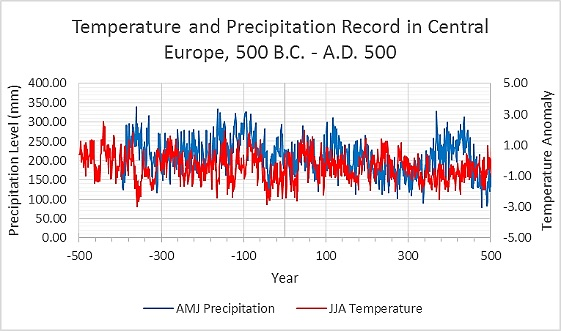
\includegraphics[width=\linewidth]{figures/Davis_Agroeconomy_Fig1.jpg}
		\centering
		\caption{Shows the April, May, June precipitation levels (AMJ) and the June, July, August temperature anomalies (JJA) between 500\BC and 500\AD. (Data source: \textcite{Büntgen_2011b}; National Climatic Data Center, \url{https://www.ncdc.noaa.gov/paleo/study/10394}), by author.}
		\label{fig:DavisFig1}
	\end{figure}	
	
	
	\begin{figure}[!p]
		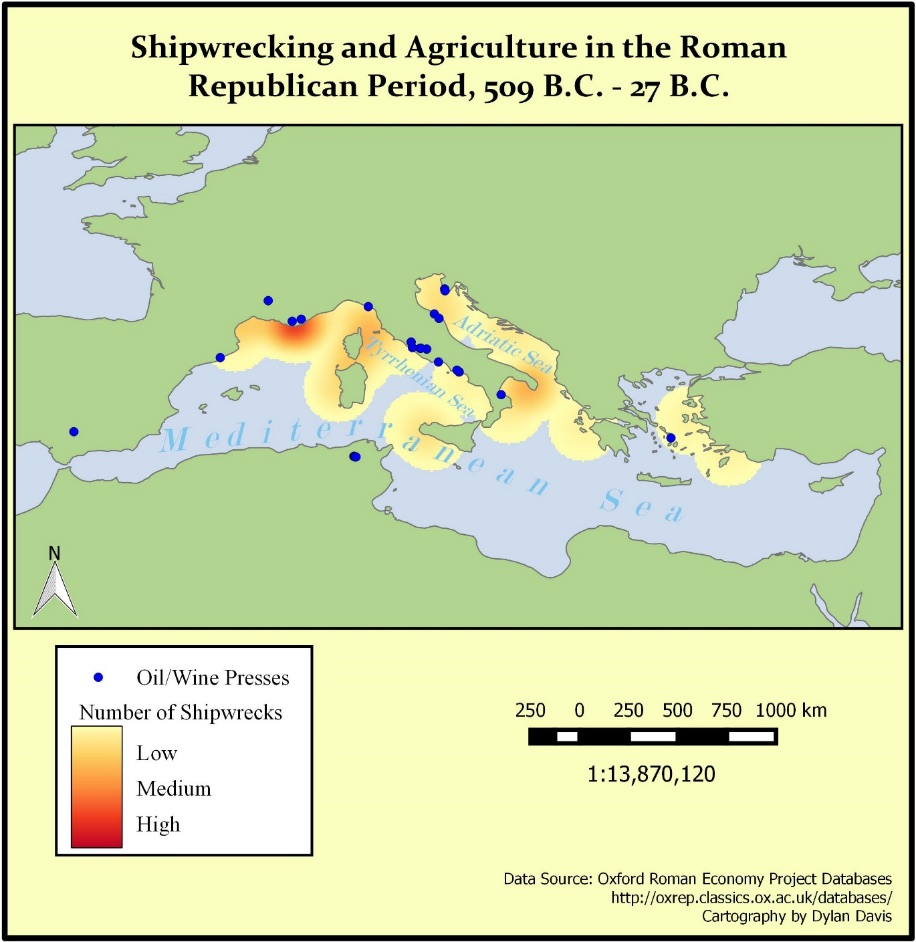
\includegraphics[width=\linewidth]{figures/Davis_Agroeconomy_Map1.jpg}
		\centering
		\caption{(Map 1) Shows the extent of maritime activity throughout the entirety of the Roman Republican Period. Note that the highest level of shipping activity seems to occur in the south of modern day France (Gaul during Roman times), by the author.}
		\label{fig:DavisMap1}
	\end{figure}
	
	
	%Map 2 or Fig 3 HERE
	
	\begin{figure}[!p]
		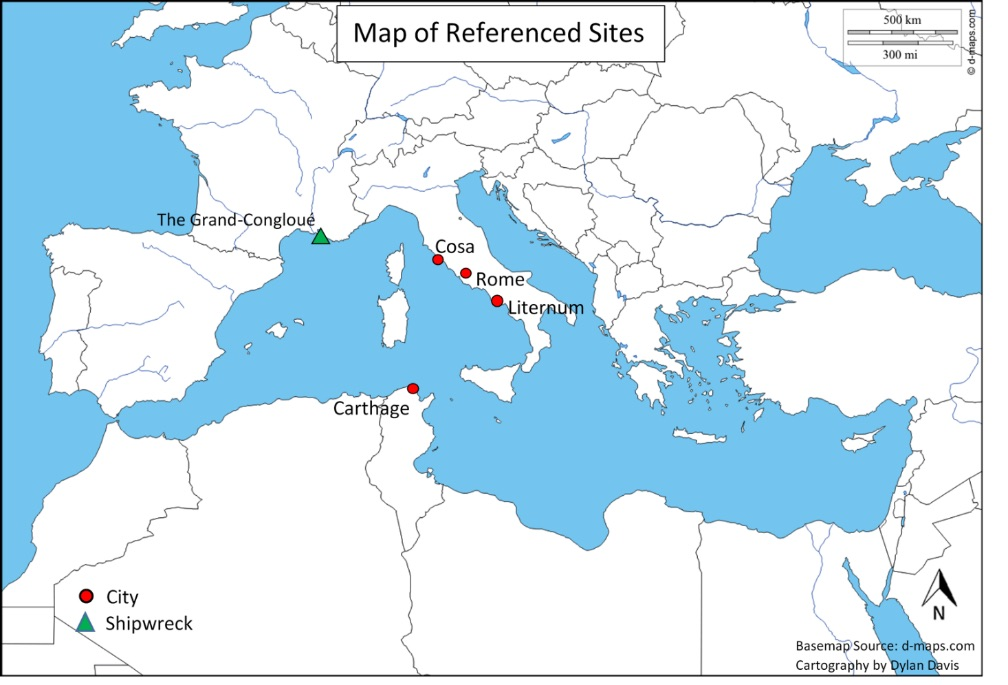
\includegraphics[width=\linewidth]{figures/Davis_Agroeconomy_Map2.jpg}
		\centering
		\caption{(Map 2) Shows all archaeological sites and locations specifically mentioned throughout the paper, by the author.}
		\label{fig:DavisMap2}
	\end{figure}
	
	
	\begin{figure}[!p]
		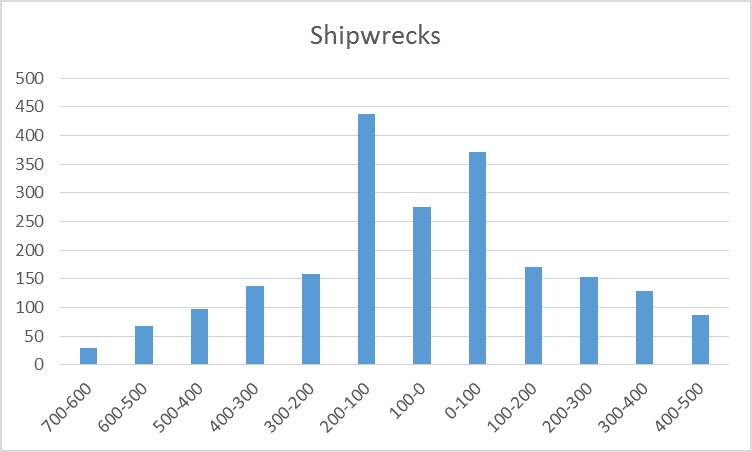
\includegraphics[width=\linewidth]{figures/Davis_Agroeconomy_Fig2.jpg}
		\centering
		\caption{Timeline of Shipwrecks in the Mediterranean from 700\protect\BC -- 500\protect\AD (Data Source: The Oxford Roman Economy Project), by the author.}
		\label{fig:DavisFig2}
	\end{figure}
	
	%Map 3 or Fig 5 HERE
	
	\begin{figure}[!p]
		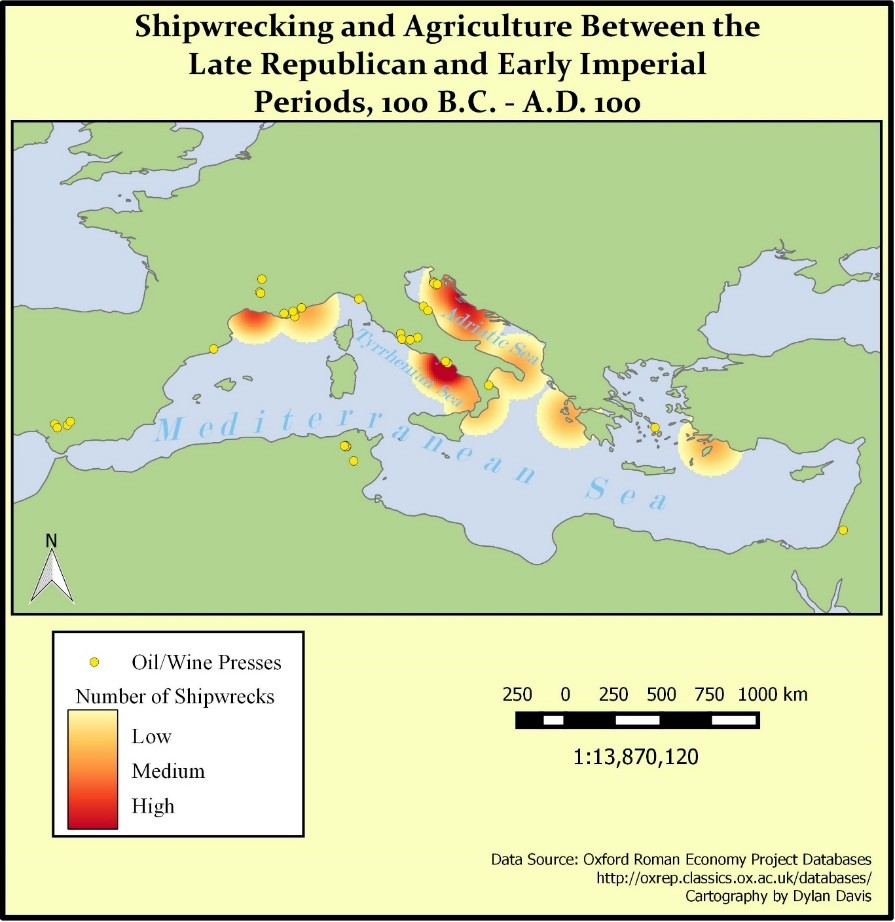
\includegraphics[width=\linewidth]{figures/Davis_Agroeconomy_Map3.jpg}
		\centering
		\caption{(Map 3) Shows the maritime activity that occurs during the transition from the Republic to the Imperial Period. Note the high levels of shipping disasters in southern Italy and modern day Croatia (in the Adriatic). In addition, Gaul continues to maintain high maritime activity.}
		\label{fig:DavisMap3}
	\end{figure}
	
	
	\begin{figure}[!p]
		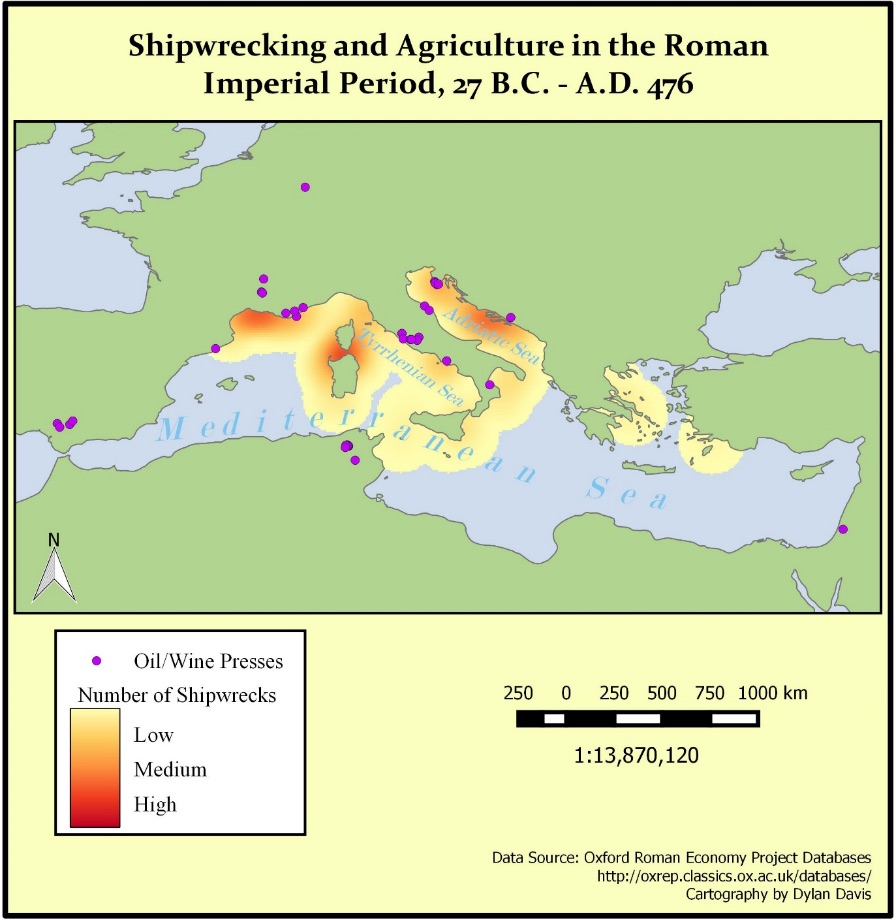
\includegraphics[width=\linewidth]{figures/Davis_Agroeconomy_Map4.jpg}
		\centering
		\caption{(Map 4) Shows maritime activity throughout the entirety of the Roman Imperial Period. Gaul remains highly active along with the islands of Sardinia and Corsica, as well as the Adriatic region, by the author.}
		\label{fig:DavisMap4}
	\end{figure}
	
	
	
	\begin{figure}[!p]
		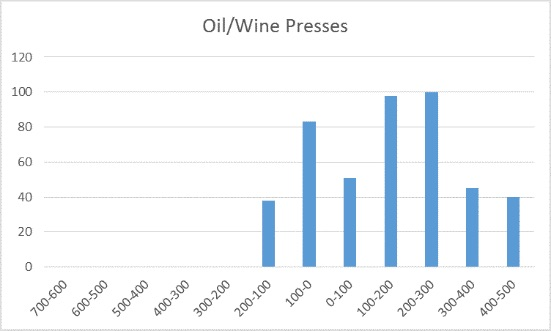
\includegraphics[width=\linewidth]{figures/Davis_Agroeconomy_Fig3.jpg}
		\centering
		\caption{Timeline of Olive Oil and Wine Presses from 700\BC –  500\AD (Data Source: the Oxford Roman Economy Project Databases), by the author.}
		\label{fig:DavisFig3}
	\end{figure}
	
	
	\begin{figure}[!p]
		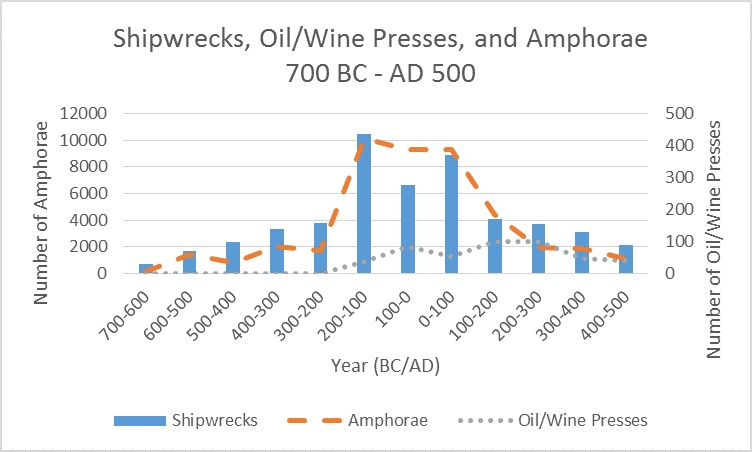
\includegraphics[width=\linewidth]{figures/Davis_Agroeconomy_Fig4.jpg}
		\centering
		\caption{The number of shipwrecks and the number of olive oil and wine presses from 400\BC – \AD 500. (Data Source: the Oxford Roman Economy Project Databases), by the author.}
		\label{fig:DavisFig4}
	\end{figure}
	
	\begin{figure}[!p]
		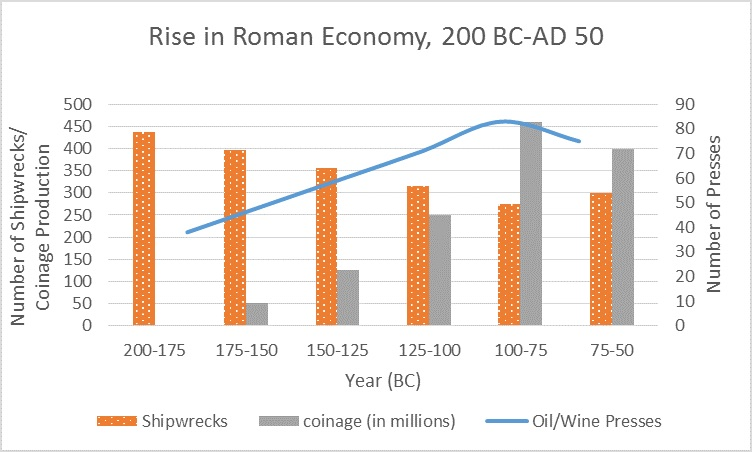
\includegraphics[width=\linewidth]{figures/Davis_Agroeconomy_Fig5.jpg}
		\centering
		\caption{Shows the increase in shipwrecks, oil and wine presses, and coinage production from 200\BC – 50\BC. Data Source: the Oxford Roman Economy Project Databases and \textcite{Hopkins_1980}, by the author.}
		\label{fig:DavisFig5}
	\end{figure}
	
	
	\begin{figure}[!p]
		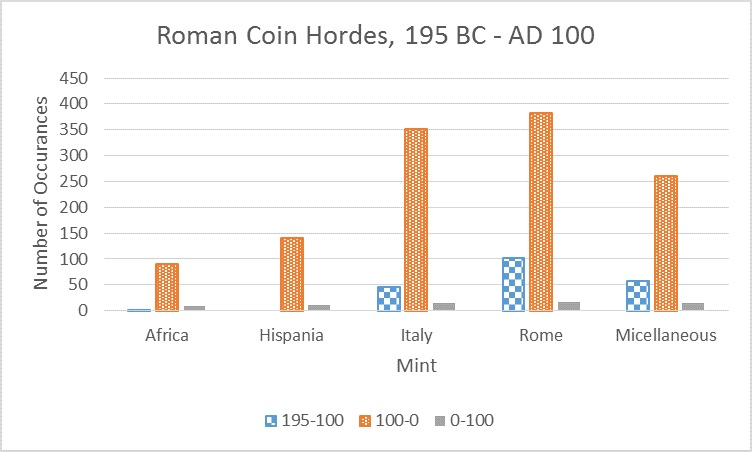
\includegraphics[width=\linewidth]{figures/Davis_Agroeconomy_Fig6.jpg}
		\centering
		\caption{Shows the level of coinage production throughout Roman territory from 195\BC – 100\AD, based on coin hordes that have been recovered. The data show a peak in coinage production in the \nth{1} century\BC. (Data from \textcite{Lockyear_2013}), by the author.}
		\label{fig:DavisFig6}
	\end{figure}
	
	
	
	\begin{figure}[!p]
		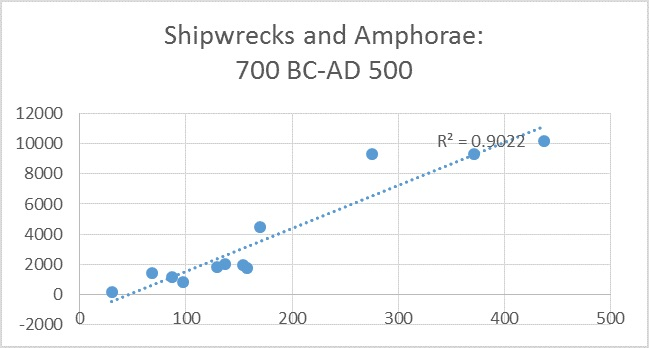
\includegraphics[width=\linewidth]{figures/Davis_Agroeconomy_Fig7a.jpg}
		\centering
		\caption{Shows the rise in the number of shipwrecks and amphorae between 700 \BC and \AD 500. There is a very strong correlation (r = \num{0.949823025}) between these two variables, suggesting a strong association. (Data Source: the Oxford Roman Economy Project Databases), by the author.}
		\label{fig:DavisFig7a}
	\end{figure}
	
	
	
	\begin{figure}[!p]
		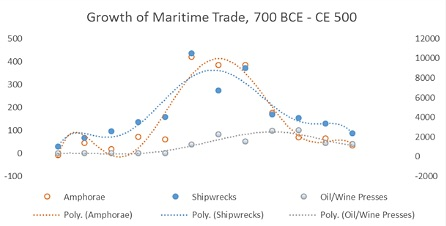
\includegraphics[width=\linewidth]{figures/Davis_Agroeconomy_Fig7b.jpg}
		\centering
		\caption{Shows the rise in the number of shipwrecks, oil and wine presses, and amphorae between 700\BC and  500\AD (Data Source: the Oxford Roman Economy Project Databases), by the author.}
		\label{fig:DavisFig7b}
	\end{figure}
	
	
	\begin{figure}[!p]
		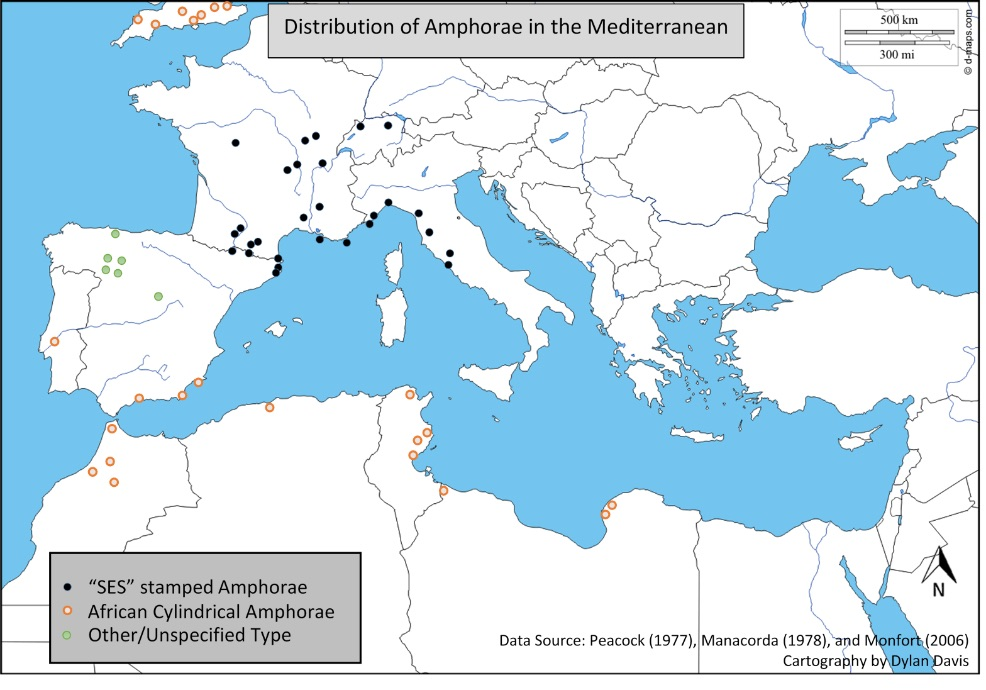
\includegraphics[width=\linewidth]{figures/Davis_Agroeconomy_Map5.jpg}
		\centering
		\caption{(Map 5) Shows the distribution of the Sestius (SES) amphorae as well as African amphorae throughout the Mediterranean region. Notice that SES amphorae disseminated throughout Western Europe (specifically Gaul). African amphorae made it all the way into Britain. After \textcite{Peacock_1977}, \textcite{Manacorda_1978}, and \textcite{Monfort_2006}, by the author.}
		\label{fig:DavisMap5}
	\end{figure}
	
	
	\begin{figure}[!p]
		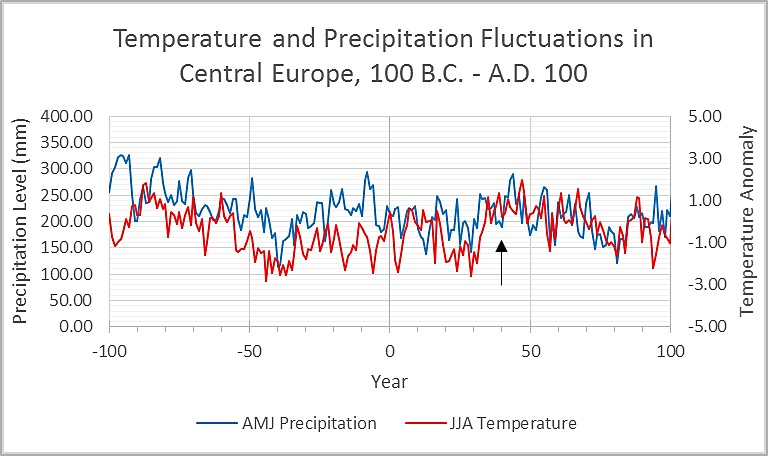
\includegraphics[width=\linewidth]{figures/Davis_Agroeconomy_Fig8.jpg}
		\centering
		\caption{Notice the gradual decrease in temperature and precipitation throughout the first half of the \nth{1} century\BC and the increase in temperature and precipitation throughout the second half of the \nth{1} century\BC The rapid warming that peaks around 40\AD  (highlighted by the arrow) is clearly noticeable. (Data source: \textcite{Büntgen_2011b}; National Climatic Data Center, \url{https://www.ncdc.noaa.gov/paleo/study/10394}), by the author.}
		\label{fig:DavisFig8}
	\end{figure}
	
	
	
	\begin{figure}[!p]
		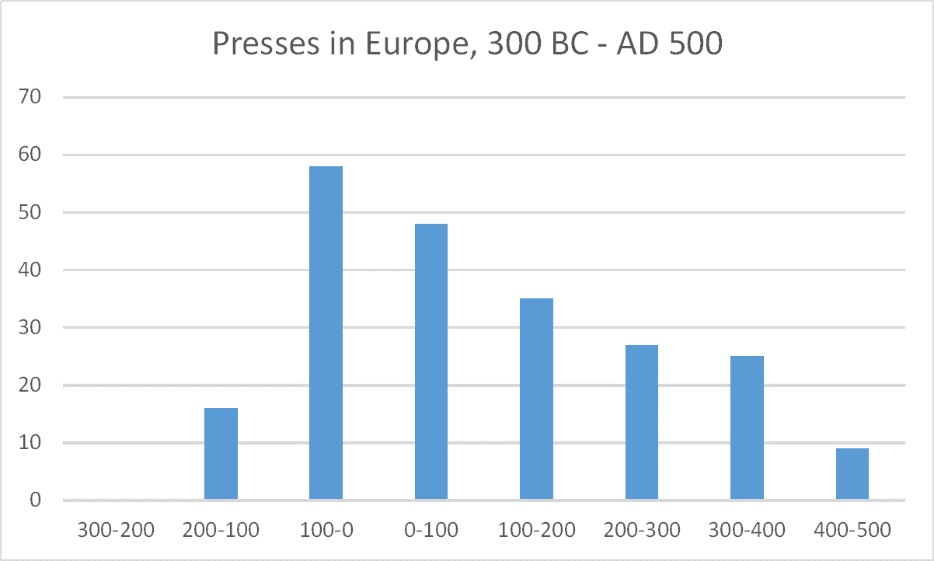
\includegraphics[width=\linewidth]{figures/Davis_Agroeconomy_Fig9.jpg}
		\centering
		\caption{Shows the number of olive oil and wine presses that were in use in the European parts of the Roman Republic/Empire from 200 \BC –  500\AD. These presses were located in Croatia, France, Greece, Italy, Portugal, and Spain. (Data from Oxford Roman Economy Databases), by the author.}
		\label{fig:DavisFig9}
	\end{figure}
	
	
	
	\begin{figure}[!p]
		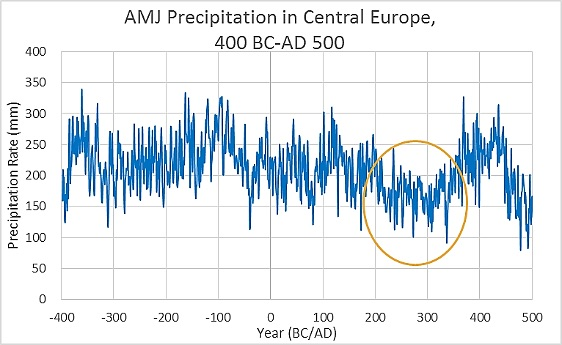
\includegraphics[width=\linewidth]{figures/Davis_Agroeconomy_Fig10.jpg}
		\centering
		\caption{Shows the April, May, June (AMJ) precipitation record in Central Europe from 400\BC – \AD 500. The orange oval highlights the distinctive drying that occurs during the \nth{2} century \AD (Data Source: \textcite{Büntgen_2011b}; National Climatic Data Center, \url{https://www.ncdc.noaa.gov/paleo/study/10394}), by the author.}
		\label{fig:DavisFig10}
	\end{figure}
	
	
	
	\begin{figure}[!p]
		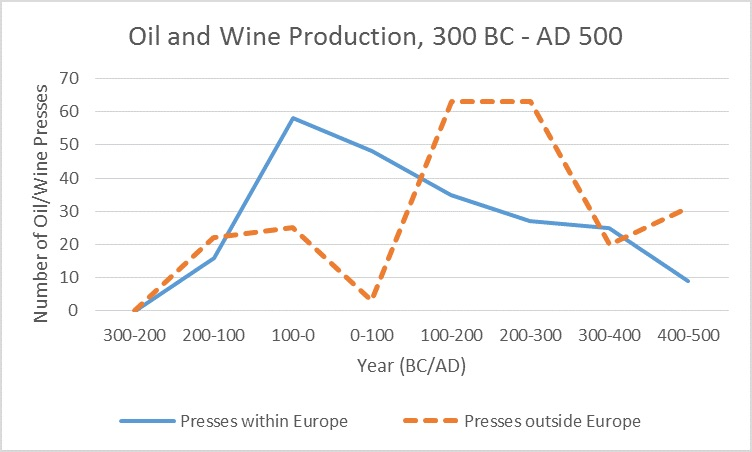
\includegraphics[width=\linewidth]{figures/Davis_Agroeconomy_Fig11.jpg}
		\centering
		\caption{Shows the number of olive oil and wine presses in use within and outside of Europe. Notice the drop in the number of presses in Europe beginning in the \nth{1} century, but the rise outside of Europe by the second century. While Europe is in a state of decline, the rest of the empire prospers, until the \nth{3} and \nth{4} centuries. (Data Source: the Oxford Roman Economy Project Databases), by the author.}
		\label{fig:DavisFig11}
	\end{figure}
\clearpage	
\myseparator
\begin{myabstract}	
	\foreignlanguage{italian}{Questo\marginnote{Abstract (Italian)} articolo esamina la relazione tra l'oscillazione del record ambientale e il successo delle istituzioni sociali nell'Impero Romano, in particolare l'economia. Attraverso un'indagine dettagliata l'ascesa dell'economia romana viene esplorata  attraverso l'uso di evidenze archeologiche e climatologiche. Il clima, come definito in questa articolo, consiste di quattro parti – clima ambientale, clima sociale, clima economico e clima politico – stabilendo così un modello climatico tetra-dimensionale. I risultati di questo studio indicano una forte relazione tra l'aumento dell'agricoltura e l'aumento del commercio marittimo durante la Repubblica romana e l'Impero Romano. Questo aumento nella produzione agricola è risultato in gran parte da una stabilità climatica in Europa, così come la temporanea tranquillità del clima politico a seguito della Fondazione di Roma. Nel corso dell'egemonia di Roma, così come la stabilità politica e sociale hanno conosciuto momenti di instabilità, lo, sviluppo economico – soprattutto nel settore agricolo – ha cambiato corso.}

	\keywords[Parole chiave]{Archeologia Classica, Economia Romana, Commercio Marittimo, Archeologia Ambientale, Archeologia Nautica.}
	
	\hspace{2em}\\\noindent%
	\foreignlanguage{french}{Cet\marginnote{Abstract (French)} article examine la relation entre les fluctuations dans l'environnement et le succès des institutions sociales dans l'Empire romain, plus précisément l'économie. Une étude détaillée, explorant la montée de l'économie romaine, est entreprise par l'utilisation de preuves archéologiques et climatologiques. La notion de climatologie, telle qu’on définit dans le présent document, se compose de quatre parties- climat environnement, climat social, climat économique et climat politique – établissant ainsi le modèle climatique tétra dimensionnel. Les résultats de cette étude indiquent une relation forte entre l'essor de l'agriculture et l'essor du commerce maritime au cours de la République romaine et de l'Empire romain. Cette augmentation de la production agricole a été en grande partie un résultat de la stabilité climatologique en Europe, ainsi que de la tranquillité temporaire du climat politique après la fondation de Rome. Comme la stabilité politique et sociale a oscillé tout au long des années de Rome au pouvoir, le développement économique – en particulier dans le secteur agricole – a également changé de cours.}

\keywords[Mots clés]{Archéologie Classique, L'économie Romaine, Le Commerce Maritime, Archéologie de L'environnement, Archéologie Nautique.}
\end{myabstract}
	



	\printbibliography[heading=subbibnumbered] 

	\label{davis:lastpage}
\closingarticle

